\section{{\texorpdfstring{\ouralgo}: Optimizing \mll for MTL}}
\label{sec:map-time}

The \map algorithm of \S\ref{sec:map} can be directly applied to
localize multiple intruders with optimal localization accuracy.
However, \map incurs prohibitive computational cost especially for a
large number of potential intruders.  In particular, note that if
there are $L$ potential locations, up to $T$ potential intruders, and
$W$ possible discrete transmit-power levels, then the
hypotheses-driven \map algorithm needs to consider $(LW)^T$
hypotheses---making its runtime complexity exponential in number of
potential intruders, and thus, making it impractical for localizing
even a moderate number of intruders present simultaneously.  In
addition, \mll also incurs a high training cost. In the following
subsections, we develop an optimized algorithm called \ouralgo based
on \map but with significantly improved computational and
training cost.
%%%%%
We start with optimizing the computation cost in \S\ref{sec:time}. In the following
  subsection \S\ref{sec:ipsn-power}, we derive a closed-form expression
  to efficiently estimate intruder's power in the {\em continuous}
  domain.  Finally, we discuss optimizing the training cost via a
  novel interpolation scheme \ildw.

%% Next, we use this result to design a computationally
%% efficient algorithm in the following section
%% 2) optimizing the \map algorithm in a way that
%% minimizes the subarea where ``simultaneous'' localization of multiple
%% intruders needs to be considered (the source of exponential
%% complexity).  The former cancels $W$ in the base and the later reduces
%% $L$ in the base.

%\subsection{Intruder Power Estimation in the Continuous Domain}
\label{sec:ipsn-power}

In this subsection, we derive a {\em closed-form} expression to estimate an
intruder's power in the continuous domain, for the special case of
single intruder and Gaussian probability
distributions~\cite{gauss}. The derived result essentially removes the
assumption of discrete power levels, and reduces the number of
hypotheses to consider by a factor of $W$. We use
this result within Procedure~1 of the previous subsection to further
optimize its time complexity and performance.

\para{Estimating Intruder Power, Given a Location.}  Consider the
special case of a single intruder in an area. In this case, each
hypothesis can be represented as \hlp, for each location $l$ and power
$p$ of the potential intruder. Let us focus on a particular location
$\lstar$ and the corresponding hypotheses \hLp. 
%%%%%
For a given observation vector \vx, we wish to estimate the power $P$
that corresponds to the hypothesis with maximum likelihood among the
hypotheses \hLp.
$$P = \arg max_p P(\hLp | \vx)$$
%%%%
The value $P$ can be computed by computing $P(\hLp | \vx)$ for
each $p$, but our goal is to derive a closed-form expression for $P$
from the given JPDs; such an expression yields power estimate in
continuous domain without computing $P(\hLp | \vx)$ for each possible
discrete $p$.

For each sensor (location) $j$, let $\pd(\vx_j | \hLP)$ represent the
probability distribution (PD) of $j$'s observations $\vx_j$ when the
intruder is at \lstar transmitting with power \pstar, the power used
at training.
%%%%%%
For a fixed \lstar and \pstar, the set of PDs $\pd(\vx_j | \hLP)$ are
equivalent to the JPDs defined in \S\ref{sec:ipsn-problem} under the
assumption of conditional independence\footnote{PD $\pd(\vx_j |
  \hLp)$ can be computed $\pd(\vx_j | \hLP)$ for any $p$, as the
  path-loss can be assumed to be independent of the transmit power,
  and JPD $\pd(\vx | \hLp)$ can be computed as product of PDs
  $\pd(\vx_j | \hLp)$ due to the conditional independence assumption.}.
%%%%%%%
%%%%%%%%
Let us assume that the above PDs are Gaussian
distributions~\cite{gauss}, and thus, can be represented as $\pd(\vx_j
| \hLP) = N(\mu_j, \sigma_j^2)$ for a given $\lstar$ and $\pstar$.
%%%%%%%%%%%%%
In the above setting, the power value $P$ that maximizes $P(\hLp | \vx)$
can actually be derived as a closed-form expression; we state the result
formally in the below lemma. 
\begin{lemma-wo-prf}
  Consider the special case of a single intruder in an area.  For a
  specific location $\lstar$ and power $\pstar$ (the only power used
  during training), let $\pd(\vx_j | \hLP)$ represent the PDs of the
  sensor observations at location $j$. Now, given the above PDs for
  various $j$ and an observation vector $\vx$, the power value
  $P = \arg max_p P(\hLp | \vx)$ is   given by: 
  $$\pstar + \frac{\sum_{j=1}^{S} \frac{\gamma}{\sigma_j^2}(x_j - \mu_j)}{\sum_{j=1}^{S} \frac{\gamma}{\sigma_j^2}},$$
  where $\gamma = \prod_{j=1}^{S} \sigma_j^2$ and S equals the number of sensors in the neighborhood of  $\ \lstar$.
  \label{lem:p}
\end{lemma-wo-prf}
The proof is in Appendix~\ref{appen:ipsn}. 
Here, we give its intuition based on a special case. 
Consider the special case wherein each $\sigma_j$ is 1 for all
$j$. In this special case, the Lemma's equation reduces to $P = \pstar
+ \frac{\sum_{j=1}^{S}(x_j - \mu_j)}{|S|}$, which implies that if each
observation $x_j$ is $c$ more than its mean $\mu_j$ then $P$ is also
$c$ more than $\pstar$. We note that the above result does {\em not}
extend to the case of multiple intruders. In short, the proof is a process of solving maximum likelihood estimation and multiple intruders introduce transcendental functions, thus cannot derive a closed-form solution.

\para{Use of Lemma~\ref{lem:p} in \ouralgo.} \eat{First, we note that,
  for the special case of a single intruder, the result of
  Lemma~\ref{lem:p} essentially allows us to determine continuous
  power value of the intruder while also reducing the overall
  computational complexity of the optimal \mll algorithm by a factor
  of $W$, the number of discrete power levels.}  For localization of
multiple intruders, Lemma~\ref{lem:p} can only be used in Procedure~1
of \S\ref{sec:time}, due to its assumption of a single intruder. In
particular, we can Procedure~1 of \S\ref{sec:time} as follows.
\begin{itemize}
\item
We replace \Rp by $R$, the maximum transmission radius.
  
\item
For each location $l$, using Lemma~\ref{lem:p}, we first compute the
power $p(l)$ such that the hypothesis \hlpl has the most likelihood
(among the hypotheses at $l$) using the observations from sensors
within a radius of $R$.
\item
Then, in the rest of the procedure, we only consider the (location,
power) pairs of the type $(l, p(l))$ for any $l$.
\end{itemize}
The rest of the Procedure~1 remains unchanged. The above change has two
benefits. First, the powers predicted in Procedure~1 are now
continuous rather than discrete. Second, the above removes the factor
of $W$ from the time complexity of \ouralgo and reduces it to
$O(LG_R\log(G_R) + G_R(G_R)^T)$ which becomes $O(L)$ if we consider
$G_R$ and $T$ to be relatively small constants.


\subsection{Optimizing Computation Time}
\label{sec:time}

\para{Basic Idea.}  Note that the \mll's exponential time complexity
is due to the exponential number of {\em combinations} of locations
and/or powers of the potential intruders. To motivate our proposed
optimized approach, consider a simple example of 2 intruders with
fixed power $p$ in a large area. Assume that the ``transmission
radius'' $r$ for power $p$ is much smaller than the area; we define
the {\em transmission radius} as the range till which the received
signal is more than a certain noise floor.
%%%%
The key observation is that if the intruders are far away (isolated)
from each other (specifically, more than $2r$ distance away), then
they could be localized independently. If the intruders are closer,
then there is a need to separate aggregated signal at some of the
sensors and hence we must apply the standard \mll algorithm {\em
  within that ``subarea''}; however, since each such subarea is small
(a disk of $2r$ radius around each possible location), the computation
time is reduced significantly. However, since we do not a priori know
the configurations of intruders, we need to consider appropriate
possibilities.

In essence, our optimized approach is a divide-and-conquer approach,
consisting of a sequence of two procedures each of which is executed
iteratively. The first procedure focuses on localizing ``isolated''
intruders (if any) independently, while the second procedure localizes
the remaining intruders---by considering all possible subareas as
suggested above. The challenge lies in modifying the \mll algorithm
for each iteration of the above procedures---as the hypotheses to
consider across iterations of the procedures are not disjoint. We now
describe each of the procedures.

\para{Procedure 1. Localize Isolated Intruders.}  Informally, in this
procedure, we localize intruders that are sufficiently separated from
other intruders. In other words, we localize intruders $x$ that are
surrounded by sensors that receive most of their received power from
$x$. More formally, we localize an intruder $x$ at location $l$ if (i)
$l$'s ``neighborhood'' has at least 3 sensors that receive most of
their power from $x$, and (ii) there are no other intruders in the
``vicinity'' of $l$. In essence, we iterate over all locations $l$,
and localize an intruder at $l$ if the above conditions are satisfied
with high enough probability, based on the readings of sensors around
$l$.
%%%%%
The precise definition of neighborhood above must depend on $x$'s
transmission radius which depends on its transmit power; however, as
$x$'s transmit power is unknown, we iterate over smaller and smaller
neighborhoods.

We now formally describe the procedure.  Let \Rp denote the
transmission radius for a transmit power of $p$. Let $R$ denote the
maximum transmission radius, i.e., $$\max_p \Rp.$$ In the below
description, we use a fractional value $f$ to define a neighborhood
and vicinity size. We start $f$ equal to 1, use a disk of radius
$f\Rp$ as a neighborhood and $R + f\Rp$ as the vicinity, and iterate
over the procedure for reduced values of $f$.
\begin{packedalpha}
	\item
	Let $f$ = 1.
	
	\item
	For each location and power pair $(l,p)$, compute $P(\hlp |
        \vxlp)$ using a form of Equation~\ref{eqn:bayes} over
        appropriate JPDs. Here:
        \begin{itemize}
          \item
         \hlp represents the hypothesis that an intruder is at
         location $l$ and using $p$ transmit power. We also implicitly
         assume that there is no other intruder present within a
         distance of $R + f\Rp$ from $l$; this ensures that the
         observations in $\vxlp$ are only due to the intruder at $l$.
         See Figure ~\ref{fig:mmap}.
         
       \item
         $\vxlp$ represents the observation vector for all sensors,
         but the sensors that are within a radius of $f\Rp$ around
         $l$ use an observation of ``residual'' received powers, as
         defined below, while the remaining sensors (outside the
         radius of $f\Rp$ around $l$) use an observation of the
         ``noise floor'' (in essence, we are ``zeroing'' the
         observations of the far-away sensors). See Figure~\ref{fig:mmap}.
         \end{itemize}
	
	\item
	Denote $(l,p)$ pairs that have $P(\hlp | \vxlp)$ higher than a
        certain threshold as {\em peaks}. If a location $l$ is a peak
        and there are no other peaks within a distance of $R + f\Rp$,
        then {\bf localize an intruder at $l$ with transmit power
          $p$.}

      \item
	For each sensor $s$, define its {\em residual received power}
          (RRP) as the total received power reduced by the sum of
        mean powers received from already localized intruders; the
        desired mean values are available from the given
        JPDs.
	
	\item
	Reduce $f$ and go back to step \#2 above, unless no new
        intruders were localized in (c) above. In our experiments, we
        used $f = 1, 1/2, 1/4$ and $1/8$.
\end{packedalpha}

\begin{figure}
	\centering
	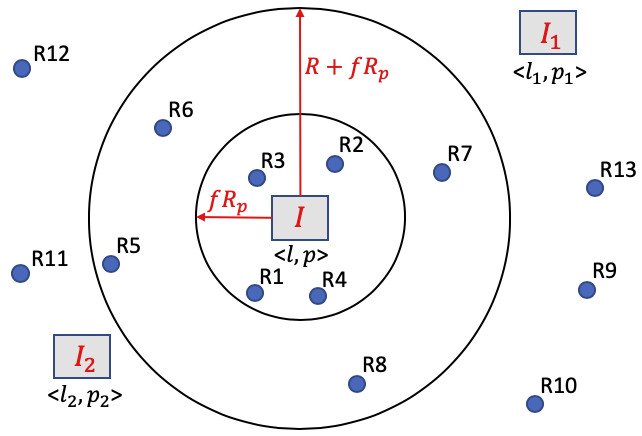
\includegraphics[width=0.7\textwidth]{chapters/ipsn/figures/mmap.png}
	\caption{Illustration of Hypothesis \hlp in Step (b) of
          Procedure~1. Here, the intruder $I$ at location $l$ is
          transmitting at power $p$, with no other intruder within a
          distance of $R + f\Rp$ from $I$. The observation vector
          $\vxlp$ consists of residual received powers from $R1$ to
          $R4$, and ``noise floor'' from the remaining sensors.}
	\label{fig:mmap}
\end{figure}

The above procedure is partly inspired by the recent localization
work~\cite{clustering}. However, instead of discarding sensors based
on their individual power and clustering the rest as
in~\cite{clustering}, we ``discard'' sensors based on their
neighborhood readings (i.e., likelihood $P(\vx| H_i)$ values) and then
``cluster'' the remaining sensors. Also, we ``cluster'' iteratively,
for smaller and smaller neighborhoods.

%% Our above procedure is partially inspired by the recent localization
%% work~\cite{clustering}, which discards sensors that receive power
%% below a certain threshold, clusters the remaining sensors, and then
%% place an intruder in each cluster. In effect, we ``discard'' a sensor
%% $s$ based on information from $s$'s neighborhood (i.e., likelihood P()
%% values) rather than $s$'s individual power as in~\cite{clustering}.
%% Also, as an improvement over~\cite{clustering}, we ``cluster''
%% iteratively, a small number of times. 
%%%%
%% Another saliant aspect of the above procedure is that we localize
%% these separated intruders based on the likelihood $P()$ function which
%% is defined for {\em each} location; in contrast, past approaches such
%% as~\cite{mobicom_utah, clustering} have localized such separated
%% intruders {\em directly} based on sensor obversations which can be
%% sparse for less dense sensor deployents and thus, yield more
%% noisy/inaccurate results.

\para{Procedure 2. Localize Intruders Situated Close-By.}  Once we
have localized separated intruders as above, we now localize remaining
intruders, if any, by applying the general \map algorithm
independently over ``subareas'' that still have some sensors with
high-enough RRP (residual received power), but no intruder localized
in the ``vicinity.'' Formally, the procedure is as follows. Let $T$ be
the maximum number of intruders allowed within a disk of radius $R$,
the maximum transmission radius.

\begin{packedalpha}
 \item
Let $s$ be the sensor with highest RRP; if $s$'s RRP is below a
certain threshold (tantamount to noise), then quit.

\item
For $t$ = 2 to $T$: Use \map (from \S\ref{sec:map}) to try to localize
$t$ transmitters within a disk of radius $R$ around $s$, using
observations of sensors within a radius of $2R$ from $s$. We use a
certain threshold for a posterior probability, in a similar way as for
Procedure~1.

\item
Update RRP of each sensor, and go to step (a) above.
\end{packedalpha}
%%%%%%%%%%%

\para{Time Complexity.} The worst-case time complexity of the first procedure is \\
$O(LWG_R\log(G_R))$, where $L$ and $W$ are the number
of potential locations (total grid cells) and transmit power levels
respectively, and $G_R$ is the maximum number of grid cells within a
transmission range of an intruder.
%%%
Here, the first term $O(LWG_R)$ is the time to compute the likelihood
values in each iteration, since the number of sensors involved in each
computation is at most $G_R$. Note that the number of iterations is
bounded by $\log(G_R)$, as $f$ is reduced by a constant multiplicative
factor.
%%%
The worst-case time complexity of the second procedure is
$O(G_R(G_R)^T)$ where $T$ is the maximum number of intruders
allowed/possible in a transmission region (i.e., a circle of radius at
most $R$).
Thus, the overall time complexity of the above localization algorithm
is $O(L.W.G_R.\log(G_R) + G_R.(G_R)^T)$.
%%%%
Generally, we would expect $T$ to be a small constant, as more than 3
intruders in a $R$-radius region with a $R$ transmission range would
interfere with each other. If we also consider $G_R$ as a small
constant, the overall time complexity can be considered to be
$O(L.W)$.  In the following subsection, we further reduce the time
complexity by removing the factor of $W$.

\subsection{Intruder Power Estimation in the Continuous Domain}
\label{sec:ipsn-power}

In this subsection, we derive a {\em closed-form} expression to estimate an
intruder's power in the continuous domain, for the special case of
single intruder and Gaussian probability
distributions~\cite{gauss}. The derived result essentially removes the
assumption of discrete power levels, and reduces the number of
hypotheses to consider by a factor of $W$. We use
this result within Procedure~1 of the previous subsection to further
optimize its time complexity and performance.

\para{Estimating Intruder Power, Given a Location.}  Consider the
special case of a single intruder in an area. In this case, each
hypothesis can be represented as \hlp, for each location $l$ and power
$p$ of the potential intruder. Let us focus on a particular location
$\lstar$ and the corresponding hypotheses \hLp. 
%%%%%
For a given observation vector \vx, we wish to estimate the power $P$
that corresponds to the hypothesis with maximum likelihood among the
hypotheses \hLp.
$$P = \arg max_p P(\hLp | \vx)$$
%%%%
The value $P$ can be computed by computing $P(\hLp | \vx)$ for
each $p$, but our goal is to derive a closed-form expression for $P$
from the given JPDs; such an expression yields power estimate in
continuous domain without computing $P(\hLp | \vx)$ for each possible
discrete $p$.

For each sensor (location) $j$, let $\pd(\vx_j | \hLP)$ represent the
probability distribution (PD) of $j$'s observations $\vx_j$ when the
intruder is at \lstar transmitting with power \pstar, the power used
at training.
%%%%%%
For a fixed \lstar and \pstar, the set of PDs $\pd(\vx_j | \hLP)$ are
equivalent to the JPDs defined in \S\ref{sec:ipsn-problem} under the
assumption of conditional independence\footnote{PD $\pd(\vx_j |
  \hLp)$ can be computed $\pd(\vx_j | \hLP)$ for any $p$, as the
  path-loss can be assumed to be independent of the transmit power,
  and JPD $\pd(\vx | \hLp)$ can be computed as product of PDs
  $\pd(\vx_j | \hLp)$ due to the conditional independence assumption.}.
%%%%%%%
%%%%%%%%
Let us assume that the above PDs are Gaussian
distributions~\cite{gauss}, and thus, can be represented as $\pd(\vx_j
| \hLP) = N(\mu_j, \sigma_j^2)$ for a given $\lstar$ and $\pstar$.
%%%%%%%%%%%%%
In the above setting, the power value $P$ that maximizes $P(\hLp | \vx)$
can actually be derived as a closed-form expression; we state the result
formally in the below lemma. 
\begin{lemma-wo-prf}
  Consider the special case of a single intruder in an area.  For a
  specific location $\lstar$ and power $\pstar$ (the only power used
  during training), let $\pd(\vx_j | \hLP)$ represent the PDs of the
  sensor observations at location $j$. Now, given the above PDs for
  various $j$ and an observation vector $\vx$, the power value
  $P = \arg max_p P(\hLp | \vx)$ is   given by: 
  $$\pstar + \frac{\sum_{j=1}^{S} \frac{\gamma}{\sigma_j^2}(x_j - \mu_j)}{\sum_{j=1}^{S} \frac{\gamma}{\sigma_j^2}},$$
  where $\gamma = \prod_{j=1}^{S} \sigma_j^2$ and S equals the number of sensors in the neighborhood of  $\ \lstar$.
  \label{lem:p}
\end{lemma-wo-prf}
The proof is in Appendix~\ref{appen:ipsn}. 
Here, we give its intuition based on a special case. 
Consider the special case wherein each $\sigma_j$ is 1 for all
$j$. In this special case, the Lemma's equation reduces to $P = \pstar
+ \frac{\sum_{j=1}^{S}(x_j - \mu_j)}{|S|}$, which implies that if each
observation $x_j$ is $c$ more than its mean $\mu_j$ then $P$ is also
$c$ more than $\pstar$. We note that the above result does {\em not}
extend to the case of multiple intruders. In short, the proof is a process of solving maximum likelihood estimation and multiple intruders introduce transcendental functions, thus cannot derive a closed-form solution.

\para{Use of Lemma~\ref{lem:p} in \ouralgo.} \eat{First, we note that,
  for the special case of a single intruder, the result of
  Lemma~\ref{lem:p} essentially allows us to determine continuous
  power value of the intruder while also reducing the overall
  computational complexity of the optimal \mll algorithm by a factor
  of $W$, the number of discrete power levels.}  For localization of
multiple intruders, Lemma~\ref{lem:p} can only be used in Procedure~1
of \S\ref{sec:time}, due to its assumption of a single intruder. In
particular, we can Procedure~1 of \S\ref{sec:time} as follows.
\begin{itemize}
\item
We replace \Rp by $R$, the maximum transmission radius.
  
\item
For each location $l$, using Lemma~\ref{lem:p}, we first compute the
power $p(l)$ such that the hypothesis \hlpl has the most likelihood
(among the hypotheses at $l$) using the observations from sensors
within a radius of $R$.
\item
Then, in the rest of the procedure, we only consider the (location,
power) pairs of the type $(l, p(l))$ for any $l$.
\end{itemize}
The rest of the Procedure~1 remains unchanged. The above change has two
benefits. First, the powers predicted in Procedure~1 are now
continuous rather than discrete. Second, the above removes the factor
of $W$ from the time complexity of \ouralgo and reduces it to
$O(LG_R\log(G_R) + G_R(G_R)^T)$ which becomes $O(L)$ if we consider
$G_R$ and $T$ to be relatively small constants.


\subsection{\ildw: Optimizing Training Cost}
\label{sec:inter}

As in supervised machine learning algorithms, our Bayesian approach
also needs training data.  We use the term
\emph{training} to denote the process of collecting data and building
up the JPDs for the hypotheses. Note that this training phase is done
only one-time,\footnote{JPDs depend on the channel state and
    hence, must be updated periodically to account for any changes in
    the environment (e.g., terrain, buildings, etc.); however, such
    environment changes are infrequent. Also, note that the
    online-training of~\S\ref{sec:auth} is done repeatedly, but only
    for specific sensors and authorized users, and thus incurs minimal
    cost. See ~\cite{mobicom19-bigspec} for spectrum sensing in both spatio and temporal domains. }
and hence, a certain cost is acceptable. The training cost
incurred during such data gathering depends greatly on the exact
mechanism used for such purposes, e.g., drones with appropriate routes
can be used to gather such data~\cite{robot-ref}.  In general, the
cost of training would depend on the number of JPDs that need to be
constructed, with the cost reduced with reduction in the number of
JPDs needed. In this subsection, we design effective {\em interpolation}
schemes that are useful in reducing the number of JPDs gathered which
in turn will reduce the overall training cost. Note that reduction in
JPDs constructed from raw data is bound to negatively impact the
accuracy---we will evaluate this trade-off in our evaluations and show
that impact on accuracy is minimal even with significant reduction in
training cost.

\para{Probability Distributions.}  First, we note that making the
following reasonable assumptions and observations can greatly reduce
the number of JPDs/PDs to be constructed.
\begin{itemize}
  \item
If we assume conditional independence of sensor observations, then
JPDs can be computed from independently constructed probability
distributions (PDs) of received powers at {\em individual sensors}.

\item
  Since received power at a sensor location $x$ due to multiple
  transmitters is merely a sum of received powers~\cite{rappaport-2001,mobicom17-splot} due to individual
  transmitters, we can compute PD at $x$ for a particular hypothesis
  involving a set $S$ of intruders from PDs due to each individual
  intruder in $S$.

\item
  Lastly, we need to only construct a PD for one transmit power for
  each transmitter and sensor location pair, since path-loss is
  independent of transmit power.
\end{itemize}
Based on the above observations, if there are $L$ discrete locations
in an area for sensors or intruders, then a \mll-based approach
requires $L^2$ PDs. Below, we propose to minimize the number of PDs to
be constructed via data gathering/training, by estimating the
remaining unconstructed PDs via interpolation.


\begin{figure}
  \center
  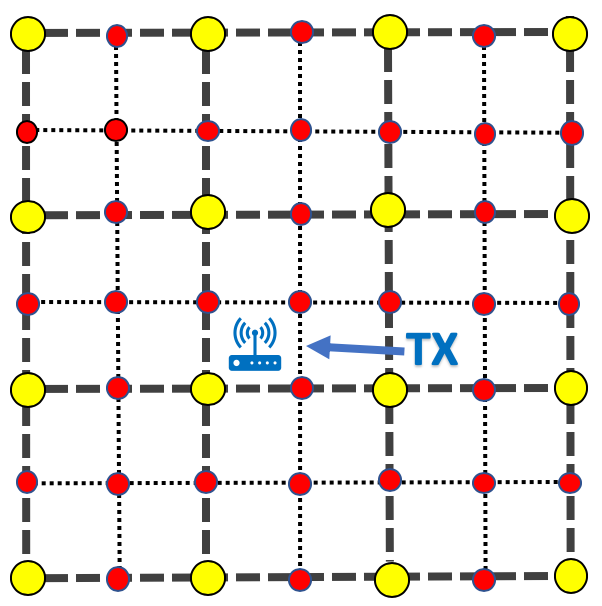
\includegraphics[width=0.45\textwidth]{chapters/ipsn/figures/multi-granular.png}
  \caption{Training for PDs at coarse-grained locations (yellow bigger
          dots), while estimating PDs using interpolation at the remaining
          fine-grained locations (red smaller dots).}
  \label{fig:path-loss}
\end{figure}

\para{Minimizing Training Cost with \ildw.} Consider a particular
location \lstar of a potential intruder. Our eventual goal is to
compute the PD for each of the $L$ possible sensor locations for this
location \lstar of a potential intruder; a PD may be computed either
by constructing it directly from gathered sensor observations or by
estimation via interpolation from the constructed PDs. In particular,
for effective interpolation, we construct PDs at coarser-grid sensor
locations, and estimate via interpolation the PDs at the remaining
finer-grid locations. See Figure~\ref{fig:path-loss}. The exact
coarseness at which the PDs are constructed is determined by the
accuracy of the interpolation scheme for a given area and/or the
impact on localization accuracy due to estimated PDs. Below, we
describe the interpolation scheme that we use for our purposes.


\begin{figure}
  \begin{subfigure}[t]{0.9\textwidth}
    \centering
    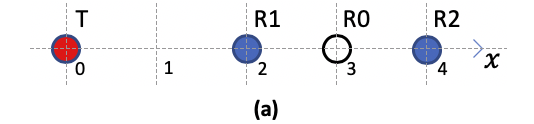
\includegraphics[width=0.5\textwidth]{chapters/ipsn/figures/interpolate.png}
  \end{subfigure}
  \qquad
  \newline
  \begin{subfigure}[t]{\textwidth}
    \centering
    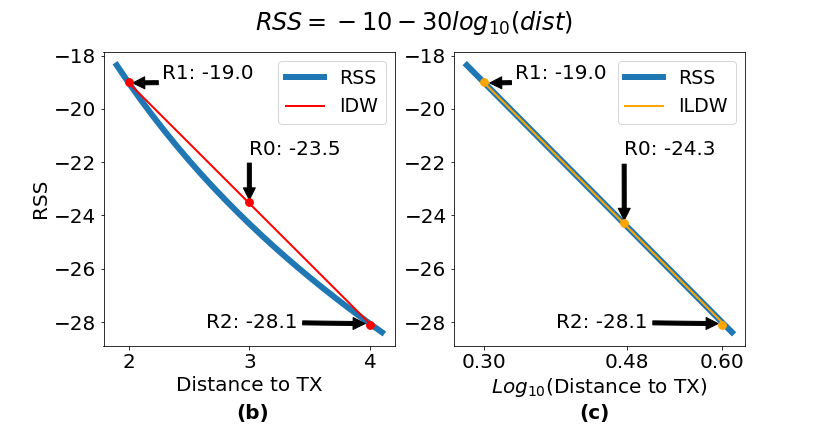
\includegraphics[width=0.8\textwidth]{chapters/ipsn/figures/ildw.png}
  \end{subfigure}
  \caption{Illustration of \ildw vs.\ IDW.
  (a) Transmitter (T), points with known (R1 and R2) and unknown (R0) received signal strength (RSS) values.
  (b) Log-normal RSS function (= -10 - 30$\log_{10}({\rm distance}))$
  plotted for varying distance from the transmitter $T$, along
  with IDW-estimated RSS value at a point between R1 and R2.
  (c) Log-normal RSS function and ILDW-estimated RSS value at
  a point between R1 and R2, plotted on a logarithmic distance
  scale.}
  \label{fig:ildw}
\end{figure}

\softpara{\ildw Interpolation Scheme.} Consider a fixed transmitter
location \lstar, and let us assume locations $\lo, \rt, \cdots, \lm$ for
which we know the path loss from \lstar. Now, consider a new point \lz
for which we wish to estimate the path-loss from \lstar.
%%%%%%%%%%%%
This is a traditional interpolation problem and well-known schemes
such as inverse distance weighting (IDW), Ordinary Kriging (OK), k-NN,
etc. have been evaluated even in the special context of signal
strength or received power~\cite{chakraborty2017specsense}.
%%%%
However, our specific context has an unique element. We
{\em know} the location \lstar of the transmitter from which the
path-loss is being estimated---as we are in the training phase wherein
we are gathering observations with transmitter at \lstar.
\eat{ (ii) Second,
the points with known values viz.\ $\lo, \rt, \cdots, \lm$ are not
arbitrary or random points, but can be chosen to facilitate accurate
estimation (e.g., in our scheme, as mentioned above, we have chosen
them to be at coarser {\em uniform} grid locations).}
%%%%%%%%
In light of the above unique element of our setting, and the observation of wireless signal characteristics, we use a custom
interpolation technique which is a nontrivial modification of the IDW
scheme, called {\em inverse log-distance weighting} (\ildw). The traditional
IDW interpolation scheme estimates the
path loss at \lz by taking a weighted average of the path-losses at
$\lo, \rt, \cdots, \lm$, with the weight being the inverse of the
distance from \lz. 
%%%%%

In our proposed \ildw scheme, we still estimate the path loss at \lz as
a weighted average of values at \li's, but assign weights differently.
In particular, we assign the weight for the point \li as the inverse
of the ``distance'' between \lz and \li in the domain where each point
is represented merely by its logarithmic distance from \lstar, the known
transmitter's location---i.e., each point $\li$ is mapped to a point
$\log d(\li, \lstar)$ on a line. This mapping is motivated by the
expectation that the actual path loss would be somewhat similar to the
log-distance path loss.
%%%%%%%
Thus, the weight for the point $\li$ is assigned to be
$$w_i = \frac{1}{|\log d(\li, \lstar) - \log d(\lz, \lstar)|},$$ where $d()$ is the
Euclidean distance function and the path loss at \lz is estimated as:
$$\uz = \frac{\sum_{i=1}^{n}w_i \ui}{\sum_{i=1}^{n}w_i},$$ where \ui
denotes the path loss at point \li from \lstar. In the above equation for
weights, if denominator is zero, then we assign $w_i$ to be equal to
the maximum of the weights among the given points (and if all
denominators are 0, each weight is assigned to be 1).
%%%%%%%
For an illustration of the above scheme, see Figure~\ref{fig:ildw}.
In the IDW scheme, \lo and \lt will get equal weights, but under the
\ildw scheme they will get weights of $5.57$ and $8.00$
respectively. More importantly, it can be easily shown that, for
log-distance path loss, \ildw estimates the path loss for \lz accurately
from two unknown points \lo and \lt, if $d(\lo, \lstar) < d(\lz,
\lstar) < d(\lt, \lstar)$.

The above discussion has been on using \ildw for estimating path-loss
values. In general, it can be easily used to estimate PDs from the PDs
at neighboring points---essentially, we can use \ildw to estimate both
the mean and standard deviation of a Gaussian PD from other means and
standard deviations respectively.
%%\red{Note that it is important
%%  to insert a known value when TX and RX are at the same location.}

%% \softpara{Interpolation Scheme.}
%% . Many interpolation schemes  exisit OK, UK, IDW.
%% . Our problem is unique in the sense that the GIVEN points for which we know the f() values can be
%%   out own choice --- in particular, we have chosen them to be uniformly distributed.
%% . We choose IDW (inverse distance weighted) due to the uniformly distributed of given points and linearity of path-loss in log-normal model.
%% . Describe IDW briefly. 
%% . We are attracted by the simplicity and effectiveness of IDW.
%% . In fact, we modify IDW for our purposes to improve its performance. We call it ILDW. 
%% explore a new interpolation method by improving IDW with the knowledge
%% of wireless propagation characteristics, name it inverse log-distance
%% weighting (ILDW).

%% The basic idea of ILDW is to
%% give hutilize the fact that the RSS is theoretically linear to the logarithm
%% of distance.

%% \para{Interpolation Schemes.}
%% Many interpolation techniques have been explored for RF signals in
%% recent works~\cite heavily borrowing works from the geospatial
%% interpolation field.  Study~\cite{sigcomm15-workshop-interpolation}
%% shows Ordinary Kriging (OK), Universal Kriging (UK) and Inverse
%% Distance Weighting (IDW) are the top 3 methods with the least
%% interpolation error. ~\cite{montero2015spatial} notes that the
%% performance of UK deteriorates largely with decrease in density of the
%% observation data samples. So OK and IDW is our choice of pick.  Both
%% OK and IDW interpolate the value at a unknown point by giving some
%% weights to the known neighboring points and average them according to
%% the weights.  The difference is how to compute the weights.  Ordinary
%% Kriging is a widely used interpolation
%% method. ~\cite{chakraborty2017specsense} improves OK by applying the
%% knowledge of wireless propagation characteristics.
%% Signal strength
%% theoretically follows a log-normal pathloss model, where the received
%% signal strength can be given by
%% \begin{equation}
%% P - 10\alpha log_{10}(d) + N(0, \delta^2)
%% \label{equ:pathloss}
%% \end{equation}
%% where $P$ is the power at the transmitter, $d$ is the distance between
%% the transmitter and point of interest, and $N(0, \delta^2)$ reflects
%% fading and shadowing affects.  \ble{[describe why we don't use
%%     kringing.]}
